\documentclass{evolang11}
\usepackage{graphicx}
\usepackage{url}
\usepackage[raggedright]{sidecap}

\begin{document}

\title{Learnability pressures influence the encoding of information density in the lexicon}

\author{Molly L. Lewis and Michael C. Frank}

\address{Psychology Department, Stanford University \\ Stanford, CA, USA \\mll@stanford.edu, mcfrank@stanford.edu}  

\maketitle



A universal feature of language is that words vary in their length within a language, in terms of morphemes, syllables, and phonemes. There have been several accounts of this variability in the literature that appeal to the form of language itself, such as the frequency of a word, or its predictability in context. Information theory, however, suggests another  factor that might influence length: the predictability, or complexity, of a word's meaning \cite{frank2008speaking}. This theory predicts that if speakers try to maintain a constant rate of information  across the speech stream, then more complex meanings should be longer. 

Previous work has shown evidence for this {\it complexity bias}. Experimentally, participants tend to assign longer words to more complex meanings, relative to shorter words \cite{lewisstructure2014}. And natural languages also show this bias \cite{lewisFrankUR}. To estimate the bias in each language, ratings of conceptual complexity were collected for 499 English words and then translated into 79 additional languages using Google Translate. For each language, there was a correlation between word length and conceptual complexity (grand mean $r =  .34$), and this bias held controlling for word frequency (grand mean $r = .22$) and other semantic variables, like concreteness. Despite the presence of this bias across all languages we examined, however, there was also a large degree of variability ($SD = .12$;  Fig.\ 1). 

 
\begin{SCfigure}[1.0][t]
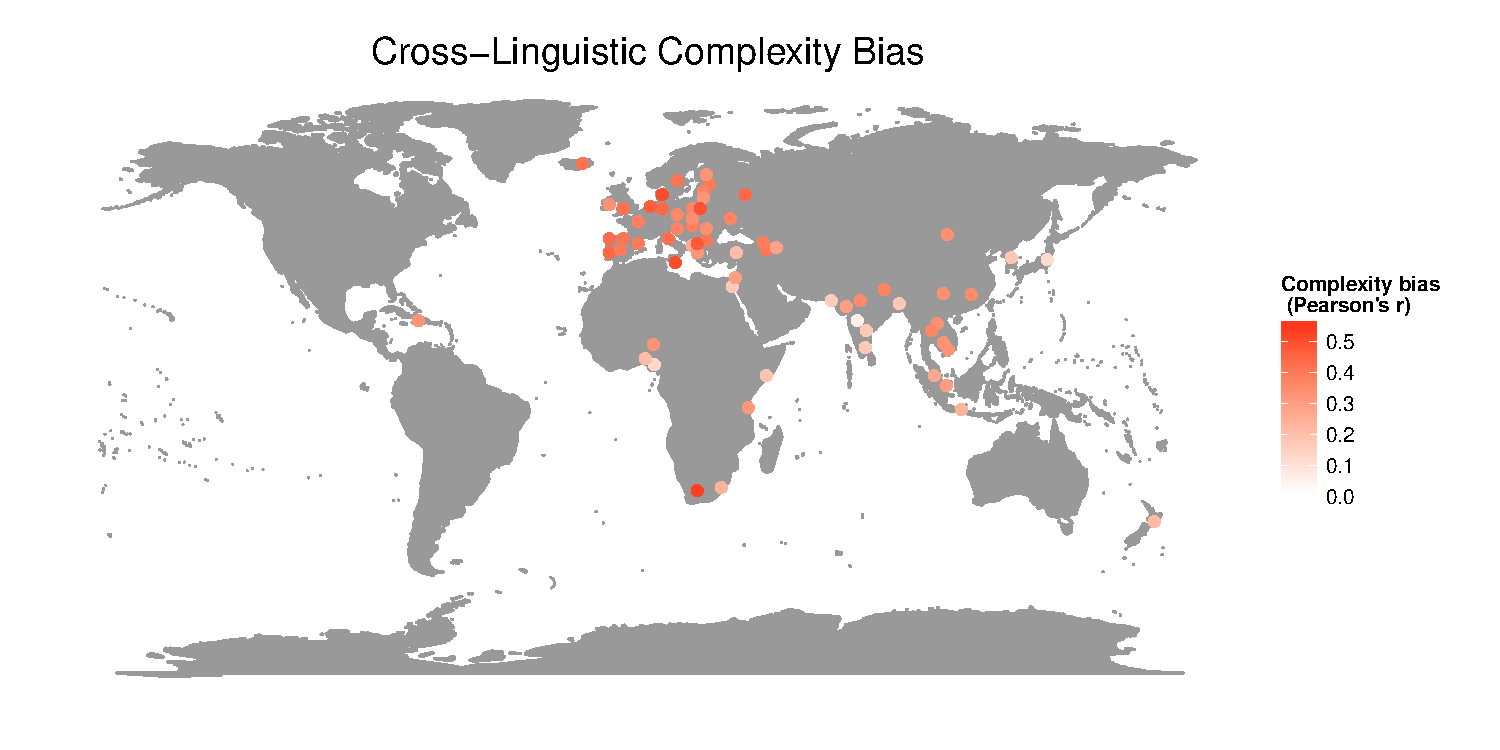
\includegraphics[width=3.1in]{Fig1.pdf}
\caption{Magnitude of the complexity bias across 79 languages. Each point corresponds to a language. \label{fig1}}
\end{SCfigure}


In our work here, we explore one possible account of this variability: that the degree to which a language encodes conceptual complexity in the lexicon is related to the learnability pressure on the language. Learnability pressure has been argued as one factor influencing the morphological complexity of a language \cite{bentz2013languages,lupyan2010language,nettle2012social}. Under this hypothesis, languages are thought to adapt to their particular social context, depending on the cohesiveness of the population acquiring the language. Languages that are  acquired by a diverse population of speakers---many adult learners, for example---might be morphologically simpler, than those acquired only by children. Consistent with this prediction, languages that are spoken by more people tend to be  morphologically simpler.

We hypothesized that the same force might influence the degree to which languages encode information density in the lexicon. We calculated the correlation between a language's complexity bias and its population of speakers. Consistent with previous work, we found that languages with more speakers tend to have a smaller complexity bias ($r = -.34$;  Fig.\ 2), and this result remained reliable even after controlling for language family. Thus, learnability pressure may force languages to rely on non-lexical strategies to maintain a uniform information density across speech.


\begin{SCfigure}[1.0][t]
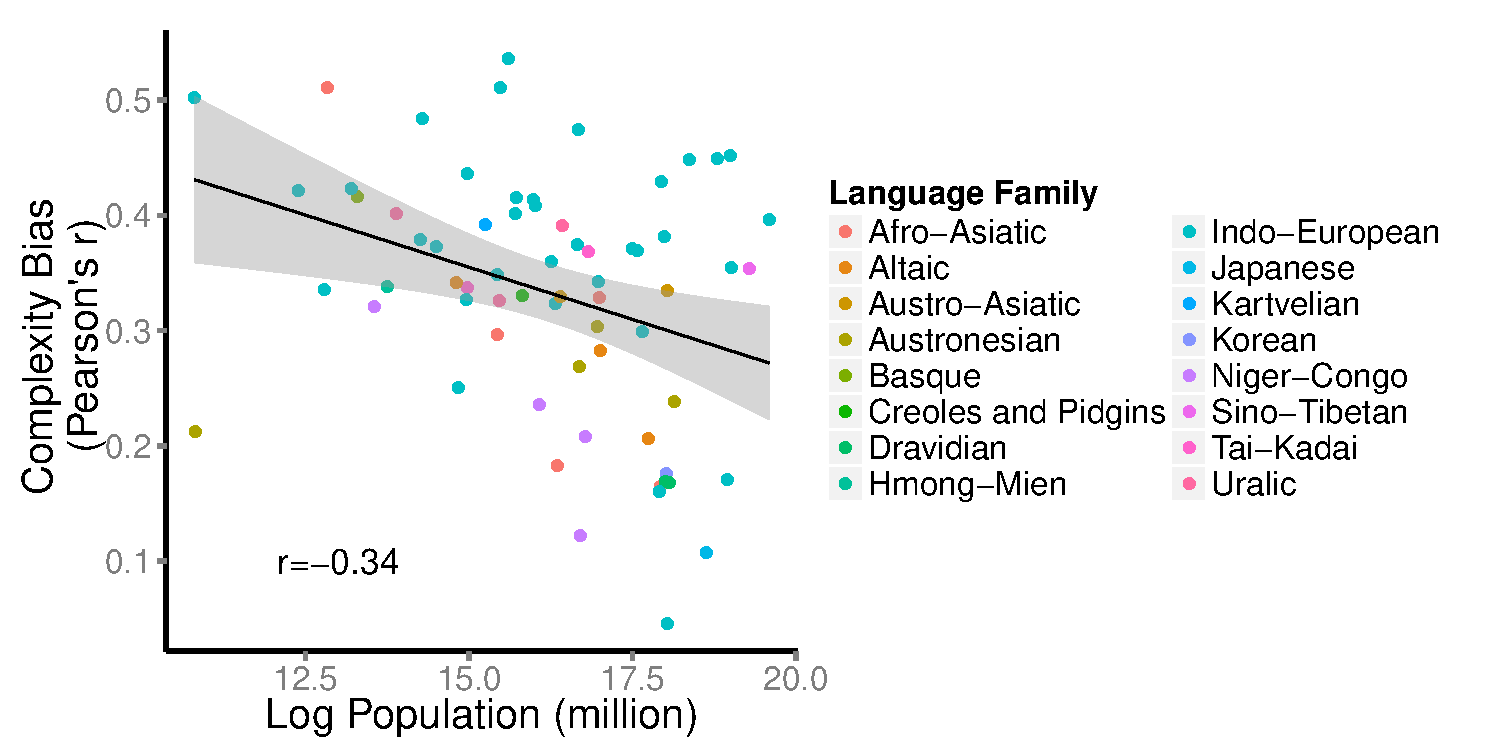
\includegraphics[width=3.2in]{Fig2.pdf}
\caption{Relationship between complexity bias and speaker population. Each point corresponds to a language. \label{fig2}}
\end{SCfigure}




\bibliographystyle{apacite}
{\footnotesize \bibliography{biblibrary} }

\end{document}
